%%%%%%%%%%%%%%%%%%%%%%%%%%%%%%%%%%%%%%%%%%%%%%%%%%%
% DOCUMENT CLASS DECLARATION
%%%%%%%%%%%%%%%%%%%%%%%%%%%%%%%%%%%%%%%%%%%%%%%%%%%
%% Use the following options:
% \documentclass[paper type% ("letterpaper" required)
% , one or two sided% ("oneside" or "twoside")%
% , font size% ("12pt" required)%
% , document type% ("these", "memoire" or "thesepararticles")%
% , document language ("francais" or "english)%
% , addition options% ("creativecommons" if the document is under the creative commons license, "hyperref", "withAlgo2e" to use algorithm2e package with proper formating)
%]{thETS}

%% Exemple with a Ph.D thesis under creative commons, using hyperref 
\documentclass[letterpaper%
, twoside%
, 12pt%
,these%
, english%
,creativecommons,hyperref%
]{thETS} 

%%%%%%%%%%%%%%%%%%%%%%%%%%%%%%%%%%%%%%%%%%%%%%%%%%%
% IMPORTANT: PRINTING WITH THE PROPER MARGINS
%%%%%%%%%%%%%%%%%%%%%%%%%%%%%%%%%%%%%%%%%%%%%%%%%%%
%% If you create a pdf with pdftex, and print it using acrobat reader, set the
%% "scaling" option to "none" to print with the proper margins.
%%%%%%%%%%%%%%%%%%%%%%%%%%%%%%%%%%%%%%%%%%%%%%%%%%%


%%%%%%%%%%%%%%%%%%%%%%%%%%%%%%%%%%%%%%%%%%%%%%%%%%%
% DECLARATION OF AN ADDITION LIST OF REFERENCES
%%%%%%%%%%%%%%%%%%%%%%%%%%%%%%%%%%%%%%%%%%%%%%%%%%%
%% Exemple of an additional list of references called "refs"
% "refs" is used as a suffix to all bibliography related commands
\newcites{refs}{LIST OF REFERENCES}

%%%%%%%%%%%%%%%%%%%%%%%%%%%%%%%%%%%%%%%%%%%%%%%%%%%
% TITLE PAGE OPTIONS
%%%%%%%%%%%%%%%%%%%%%%%%%%%%%%%%%%%%%%%%%%%%%%%%%%%

\title{Document title}

\author{First name LAST NAME}
\authorcopyright{First name Last name}

\datesoutenance{"Defense date"}

\datedepot{"Deposit Date"}

\directeur{M. }{First Name Last Name}{Department and institution}

%\directeur{Mrs.}{Prénom Nom}{Nom du département et institution}

\codirecteur{Mrs.}{First Name Last Name}{Department and institution}

%\codirecteurB{M.}{Prénom Nom}{département et institution}

\president{M.}{First Name Last Name}{Department and institution}

\examinexterne{M.}{First Name Last Name}{Department and institution}

%\jury{Mme.}{Prénom Nom}{département et institution}{}


%%%%%%%%%%%%%%%%%%%%%%%%%%%%%%%%%%%%%%%%%%%%%%%%%%%
% CHANGING THE NAME OF THE DIPLOMA
%%%%%%%%%%%%%%%%%%%%%%%%%%%%%%%%%%%%%%%%%%%%%%%%%%%
%% It is possible to change the name of the diploma by redefining
% the command \lediplome, as follows:

%\renewcommand{\lediplome}{
%    MASTER IN ELECTRICAL ENGINEERING\\M.Sc.A.
%    }

\listfiles

%%%%%%%%%%%%%%%%%%%%%%%%%%%%%%%%%%%%%%%%%%%%%%%%%%%
% ACTUAL DOCUMENT
%%%%%%%%%%%%%%%%%%%%%%%%%%%%%%%%%%%%%%%%%%%%%%%%%%%
\begin{document}

\pagenumbering{Roman}

%%- Title page -%%
\maketitle

%%- Jury presentation -%%
\presentjury

%%- Foreword -%%
\begin{foreword}

\lipsum[1] % Texte de remplissage pour donner un exemple de la mise en page

\end{foreword}



%%- Acknowledgements -%%
\begin{acknowledgements}

\lipsum[1] % Text filling, to have an example of the layout


\end{acknowledgements}


%%- Summary -%%

\begin{summary}{French title}{mot-clé1, mot-clé2}

\lipsum[1] % Text filling, to have an example of the layout

\end{summary}


%%- Abstract -%%
\begin{abstract}{keyword1, keyword2}

\lipsum[1] % Text filling, to have an example of the layout

\end{abstract}


%%- Table of contents -%%
\tableofcontents


%%- List of tables -%%
\listoftables


%%- List of figures -%%
\listoffigures


%%- List of abbreviations -%%
\begin{listofabbr}[3cm]
\item [ETS] École de Technologie Supérieure
\item [ASC] Agence Spatiale Canadienne
\end{listofabbr}


%%- List of symbols -%%
\begin{listofsymbols}[3cm]
\item [$\textbf{a}$] Première lettre de l'alphabet
\item [$\textbf{A}$] Première lettre de l'alphabet en majuscule
\end{listofsymbols}


\cleardoublepage

\pagenumbering{arabic}

% Marginpar to the left of the document
\reversemarginpar

%%%%%%%%%%%%%%%%%%%%%%%%%%%%%%%%%%%%%%%%%%%%%%%%%%%
% THESIS EXAMPLE
%%%%%%%%%%%%%%%%%%%%%%%%%%%%%%%%%%%%%%%%%%%%%%%%%%%

\begin{introduction}

\lipsum[1] % Text filling, to have an example of the layout

% Figure example
\begin{figure}
	\centering % Figures must be centered
	\fbox{ % Figures must be delimited by a rectangle
		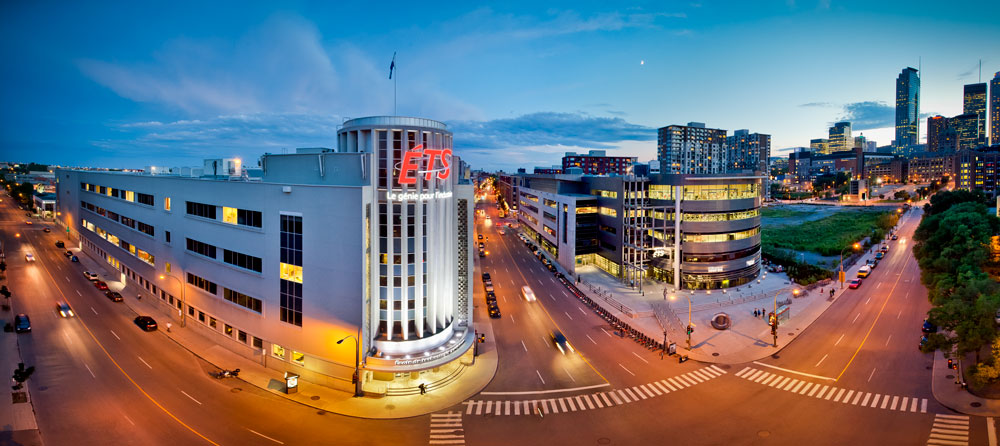
\includegraphics[width=0.75\textwidth]{Figures/vueEts.jpg} % Usage of the "width" parameter to constraint the with of the figure, respecting proportions. In this example, the width is set to 0.75 times the maximum text width (\textwidth), respecting the margins.
	}
	 \\ \parbox{0.75\textwidth}{\caption{Test of a long caption, using a framebox and a parbox to constrain the caption.}\label{fig:vueEts}} % Usage of a parbox to contrain the width of the caption, in this example fixed to the same width than the figure (0.75\textwidth). The decanat wants to avoid captions larger than the figure, if possible (i.e. if the figure is not too narrow, otherwise the caption would require too many lines) 
\end{figure}

\lipsum[1] % Text filling, to have an example of the layout


\end{introduction}

%%- Uncomment the literature review for a thesis by articles -%%
%\chapter{Literature review}


%%- First demo chapter -%%
\chapter{Long chapter tite, with linebreak. Lorem ipsum dolor sit amet, consectetur adipiscing elit. Pellentesque justo justo, porta sagittis feugiat eget, ornare rhoncus ligula. Nunc non odio sed lacus rutrum rhoncus.}


\section{Layout tests}

In this sections, several environments are presented. 

\subsection{Listing tests}

Presentation of the main listing environments: enumerations and lists.

\subsubsection{Enumerations: enum environment}

Enum environment test:
\begin{enumerate}
 \item test 1
 \item test 2
\end{enumerate}

\subsubsection{Lists: itemize environment}

Test of the itemize environment 
\begin{itemize}
 \item test 1
 \item test 2
\end{itemize}

\subsection{Equations tests}

Layout of the equations:

\begin{equation}
   \beta = 8
\end{equation}

\begin{equation}
   \gamma = \alpha \times 3
\end{equation}

\section{Second section}

Example of a second section, to test the layout in the table of contents.


%%- Second demo chapter -%%
\chapter{Second Chapter}

\section{Table layout tests}

Tables have the same constraints than the figures, except for the caption that has to be on top.


\begin{table}
		\parbox{0.65\textwidth}{\caption{Test of a long table caption, with linebreak.}} % Contrainte manuelle de la largeur de la légende
		\begin{tabular}{|c|c|c|c|c|c|c|c|}
		\hline
			{\bf titre} & {\bf titre} & {\bf titre} & {\bf titre} & {\bf titre} & {\bf titre} & {\bf titre} & {\bf titre} \\
	  \hline
			blá & blá & blá & blá & blá & blá & blá & blá \\
	  \hline
			blá & blá & blá & blá & blá & blá & blá & blá \\
	  \hline
			blá & blá & blá & blá & blá & blá & blá & blá \\
	  \hline
			blá & blá & blá & blá & blá & blá & blá & blá \\
	  \hline
			blá & blá & blá & blá & blá & blá & blá & blá \\
	  \hline
			blá & blá & blá & blá & blá & blá & blá & blá \\
	  \hline
		\end{tabular}
\end{table}


\section{References test}

\subsection{References to the bibliography}

Reference from the bibliography \cite{Arica2002}.

\subsection{References to the list of references "refs"}

References from the list of references "refs", declared at the beginning of the document \citerefs{Test}.

\subsection{References to a label of the document}

Reference to a Figure associated to a label: Figure \ref{fig:vueEts}.

\subsection{URL references}

\subsubsection{Test of "href"}

Href is used to integrate a link to a text:
\href{http://www.etsmtl.ca/Etudiants-actuels/Cycles-sup/Realisation-etudes/Guides-gabarits}{Link to the template page.}.

\subsubsection{Test de url}

Url is used to format a clickable link:
\url{http://www.etsmtl.ca/Etudiants-actuels/Cycles-sup/Realisation-etudes/Guides-gabarits}.

%%- Third demo chapter -%%
\chapter{Example of a thesis by article, with integrated article}

% \articleAuthors{Names}{Affiliations} is used to print authors and their affiliations. Names must be declared as {First name1 Last Name1}{First Name2 Last Name2}... , as well as the affiliations
%Exemple \articleAuthors{{First Name Last Name}}{{Affiliation}}

\articleAuthors{
{First name Last name\textsuperscript{1}}{First name Last name\textsuperscript{1}}
}{
{\textsuperscript{1} Département de Génie Mécanique, École de Technologie Supérieure,\\
1100 Notre-Dame Ouest, Montréal, Québec, Canada H3C 1K3\\
Article soumis à la revue « Vecteur environnement » en septembre 2010.}
}

\section{Section 1}

\lipsum[1] % Text filling, to have an example of the layout

%%- Conclusion -%%
\begin{conclusion}

\lipsum[1] % Text filling, to have an example of the layout

\end{conclusion}


%%%%%%%%%%%%%%%%%%%%%%%%%%%%%%%%%%%%%%%%%%%%%%%%%%%
%  Appendix example:
%%%%%%%%%%%%%%%%%%%%%%%%%%%%%%%%%%%%%%%%%%%%%%%%%%%
\appendix

%% To use more than one appendix
\multiannexe

%% Appendix from an external file
% \include{extApp}

\chapter{Appendix example} 


\section{First section of the appendix}


\subsection{Figures in annexes}

\begin{figure}
	\centering
	\fbox{
		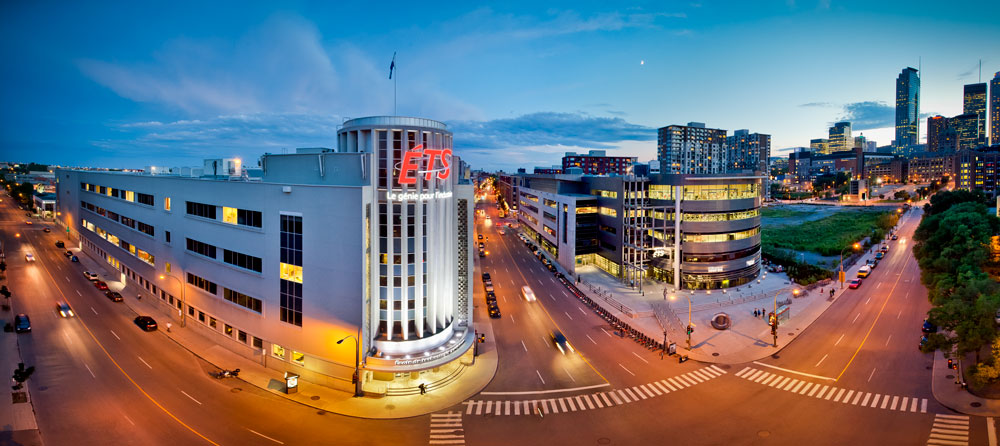
\includegraphics[width=0.75\textwidth]{Figures/vueEts.jpg}
	}
	 \\ \parbox{0.75\textwidth}{\caption{Figure in an appendix.}\label{fig:testAp}}
\end{figure}

In the annexes, the figures are declared in the same way. Their numbering changes automatically (e.g. Figure \ref{fig:testAp}).

\subsubsection{Tables in annexes}

\begin{table}
		\parbox{0.65\textwidth}{\caption{Table in an appendix.}\label{tab:testAp}}

		\begin{tabular}{|c|c|c|c|c|c|c|c|}
		\hline
			{\bf titre} & {\bf titre} & {\bf titre} & {\bf titre} & {\bf titre} & {\bf titre} & {\bf titre} & {\bf titre} \\
	  \hline
			blá & blá & blá & blá & blá & blá & blá & blá \\
	  \hline
			blá & blá & blá & blá & blá & blá & blá & blá \\
	  \hline
			blá & blá & blá & blá & blá & blá & blá & blá \\
	  \hline
			blá & blá & blá & blá & blá & blá & blá & blá \\
	  \hline
			blá & blá & blá & blá & blá & blá & blá & blá \\
	  \hline
			blá & blá & blá & blá & blá & blá & blá & blá \\
	  \hline
		\end{tabular}
\end{table}

Same behaviour for the tables (e.g., Table \ref{tab:testAp}).


%%%%%%%%%%%%%%%%%%%%%%%%%%%%%%%%%%%%%%%%%%%%%%%%%%%
% BIBLIOGRAPHY AND REFERENCES
%%%%%%%%%%%%%%%%%%%%%%%%%%%%%%%%%%%%%%%%%%%%%%%%%%%

%%- Bibliography -%%
\newpage
% Single spacing for the bibliography
\begin{spacing}{1}  
	\nocite{*} % The "nocite" command can be used to print references that haven't been used in the document. The "*" option specifies that every reference should be printed
	\bibliographystyle{bibETS} % ETS bibliography style
	\addcontentsline{toc}{chapter}{BIBLIOGRAPHY} % Addition of the bibliography in the table of contents
	
	\bibliography{biblio} % List of bibliography files, biblio.bib is an example
	
\end{spacing}

%%- Other list of references, "refs" example --%
%%%%%%%%%%%%%%%%%%%%%%%%%%%%%%%%%%%%%%%%%%%%%%%%%%%
% IMPORTANT: HOW TO COMPILE AND PRINT ADDITIONAL REFERENCES (replace "refs" by the chosen name)
%%%%%%%%%%%%%%%%%%%%%%%%%%%%%%%%%%%%%%%%%%%%%%%%%%%
% Follow these three steps:
%   1. Compile the document once, to save the used references in refs.aux 
%   2. Compile the references
% 		- On Linux: Use the "bibtex refs" command in the document folder
%		- On MacOSX (MacTex distribution): Use the "/usr/texbin/bibtex refs" command in the document folder	
%		- On Windows: Edit the "update_refs.bat" script to put the right suffix ("refs" here), and launch the script
%   3. Recompile the document TWICE
%%%%%%%%%%%%%%%%%%%%%%%%%%%%%%%%%%%%%%%%%%%%%%%%%%%

\newpage
% Same commands than for the bibliography, only with the "refs" suffix
\begin{spacing}{1} 
	%\nociterefs{*}
	\bibliographystylerefs{bibETS}
	\addcontentsline{toc}{chapter}{LIST OF REFERENCES}

	\bibliographyrefs{refs}
	
\end{spacing}

\end{document}
